\documentclass[10pt]{article}
\usepackage{graphicx}
\usepackage[margin=1.5cm]{geometry}
\usepackage{amsmath}
\def\brcurs{{\mbox{$\resizebox{.16in}{.08in}{
\includegraphics{BoldR}}$}}}
\def\rcurs{{\mbox{$\resizebox{.16in}{.08in}{
\includegraphics{ScriptR}}$}}}

\begin{document}
\twocolumn

\title{Tuesday Warm-up: Lorentz Force Law, and Biot-Savart Law}
\author{Prof. Jordan C. Hanson}

\maketitle

\section{Memory Bank}

\begin{itemize}
\item \textbf{Lorentz force}:
\begin{equation}
\mathbf{F} = Q(\mathbf{E} + \mathbf{v} \times \mathbf{B})
\end{equation}
\item \textbf{Position for uniform circular motion} \textit{(xy-plane)}:
\begin{equation}
\mathbf{r}(t) = |\mathbf{r}|\cos(\omega t)\hat{i} + |\mathbf{r}|\sin(\omega t)\hat{j}
\end{equation}
\item \textbf{Centripetal force}:
\begin{align}
\mathbf{F}_{\rm C} &= -m r \omega^2 \hat{\mathbf{r}} \\
\mathbf{F}_{\rm C} &= -m v^2 r^{-1} \hat{\mathbf{r}}
\end{align}
\item \textbf{Mass and charge of proton}:
\begin{align}
q &= 1.602 \times 10^{-19}~~C \\
m &= 1.673 \times 10^{-27}~~kg
\end{align}
\end{itemize}

\begin{figure}
\centering
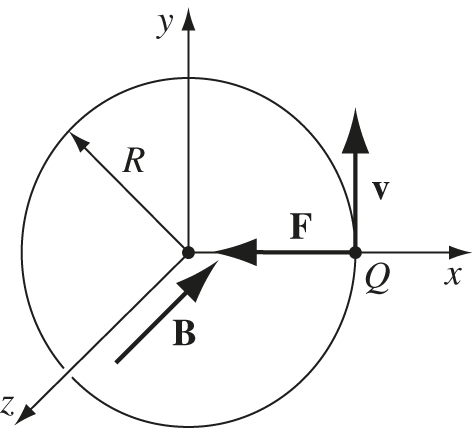
\includegraphics[width=0.2\textwidth]{figures/5_4.jpg} \hspace{0.5cm}
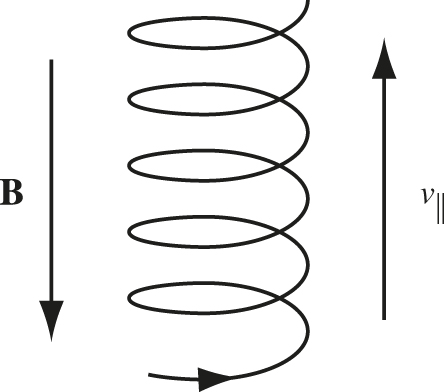
\includegraphics[width=0.2\textwidth]{figures/5_5.jpg}
\caption{\label{fig:1} (Left) Uniform circular motion of a charge $Q$ within a magnetic field $B$. (Right) Helical motion within a field, with average velocity $v_{||}$.}
\end{figure}

\section{Lorentz Force}

\begin{enumerate}
\item Consider Fig. \ref{fig:1} (left).  (a) Show that, if $\mathbf{E} = 0$, the motion is circular, with constant frequency
\begin{equation}
\omega_{\rm C} = \frac{qB}{m}
\end{equation}
The parameter $\omega_{\rm C}$ is known as the \textit{cyclotron frequency}.  (b) What is $\omega_{\rm C}$ for a proton circling in a 1 Tesla magnetic field? (c) Suppose $\mathbf{r}(0) = 1.0\hat{i}$ m.  Where is the proton at $t=7.83$ ns? (d) If the proton moves along the z-axis with $v_z = 0.003$ m ns$^{-1}$, what is the position at 2.61 ns?  The motion is depicted in Fig. \ref{fig:1} (right).  \\ \vspace{3.5cm}
\item A particle of charge $q$ enters a region of uniform field $\mathbf{B}$ (pointing \textit{into} the page).  The field deflects the particle a distance $d$ above the original line of flight (Fig. \ref{fig:2}). (a) Is the charge negative or positive? (b) In terms of $a$, $d$, $B$, and $q$, find the momentum of the particle. \\ \vspace{3cm}
\item In 1897, J.J. Thomson first measured the charge-to-mass ratio of electrons.
\begin{itemize}
\item First he passed the beam of cathode rays through uniform crossed $\mathbf{E}$ and $\mathbf{B}$ fields.  These were mutually perpendicular, and both perpendicular to the beam. He adjusted the $\mathbf{E}$ field until he got zero deflection.  What was the speed of the electrons, in terms of $\mathbf{E}$ and $\mathbf{B}$?
\item Then he turned off $\mathbf{E}$ and measured the radius of curvature $R$ of the beam.  In terms of $E$, $B$, and $R$, what is $(q/m)$ for the beam?
\end{itemize}
\end{enumerate}

\begin{figure}
\centering
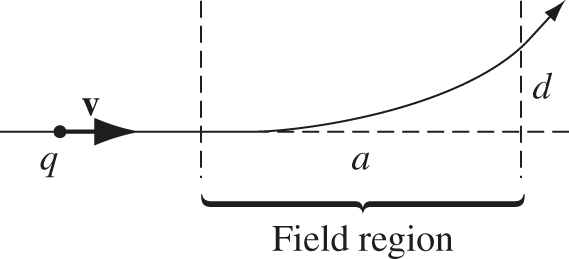
\includegraphics[width=0.35\textwidth]{figures/5_7.jpg}
\caption{\label{fig:2} A charge passes through a region with a $\mathbf{B}$-field \textit{into} the page.}
\end{figure}

\end{document}
